\documentclass{article}

\usepackage[final]{neurips_2023}
\usepackage{amsmath,amssymb}
\usepackage{tikz}
\usepackage{graphicx}
\usepackage{float}
\usetikzlibrary{arrows.meta,positioning}

% narrower margins (wider text block)
\AtBeginDocument{
  \newgeometry{
    textheight=9in,
    textwidth=7in,
    top=1in,
    headheight=12pt,
    headsep=25pt,
    footskip=30pt
  }
}

% remove NeurIPS footer on first page
\makeatletter
\renewcommand{\@notice}{}
\makeatother

\title{Transfer Learning Project: Two-Headed CNN with Interaction Loss}

\author{
Christian Montgomery and Aksel Kretsinger-Walters \\
Columbia University \\
\texttt{cm4521@columbia.edu, adk2164@columbia.edu}
}

\begin{document}

\maketitle
\vspace{-3em} % tighten space before Introduction

\section{Introduction}

In order to maximize performance / minimize error on the Transfer Learning project, we are going to construct a 2-headed CNN to learn the sub-class and super-class classifications. We plan to do this both for our own model trained from the ground up, and also on top of a pretrained image recognition model to compare performance. In order to ensure our model generalizes well to unseen categories, we are going to augment our training dataset with various image types not in sample (subset of the ImageNet $\sim$ 20,000 categories) and modify our training set images (translate, vertical/horizontal flip, rotations, etc.).  In addition, we will incorporate various methods (through trial and error) to improve generalization discussed in class such as regularization penalty/weight decay, early stopping, adding linear bottleneck layers and implementing dropout of units. Lastly, we plan on experimenting with an ensemble of models (bagging/boosting) to maximize our model performance on the class leaderboard.

\section{Method / Algorithms to investigate}

To initially normalize our input data, our plan is to rescale each pixel value to between [0, 1] for each input channel (RGB). Once we introduce data augmentation to the training data, we may also use batch normalization to Z-score across mini-batches to decrease training speed.

From the provided training data, we plan on performing data augmentation to ensure our model is able to generalize well. This includes extending our training set with modifications to original training images, such as horizontal/vertical flipping, rotations, translation, and noise. In addition to the provided training data, we plan on curating a subset of ImageNet representative of the wide variety of various other categories beyond the 3 provided. Thus, we will train our model to recognize any of these other broad categories as “novel” superclass. Then we plan to pull a small subset of images representing other subcategories of reptiles, birds, and dogs so that our model can identify “novel” subclasses (perhaps 10 examples per new subcategory).

We've decided to use a convolutional neural network as our base model as convolutions have been repeatedly shown to perform well on image classification tasks. In order to keep the number of parameters down, we plan on combining the CNN with linear bottleneck layers.

To ensure our CNN is robust, we plan on incorporating pooling, residual layers (skip-layer connections) and ReLU activation functions to help overcome the vanishing gradient problem. We also plan to use a weight initialization method to break symmetry during training

In order to have full control over the weights learned of our model, we will first training our own CNN from scratch. Then, separately we will take a pretrained model as a base (i.e. ResNet, AlexNet), freezing weights and then fine-tuning on our specific transfer learning problem. Our aim is to compare performance between these two approaches, and potentially combine them.

After the CNN backbone to learn a feature vector for the image, we have decided upon having 2-separate heads, one for each class category (superclass and subclass). We’ve decided to try this first instead of 2 distinct models, for simplicity and time efficiency of training. For each head, we will learn weights for that linear layer, and calculate cross-entropy loss via calculating logits and softmax for each potential superclass \& subclass respectively.

However, we are aware of potential divergence between superclass and subclass predictions (for example, if the superclass prediction is bird but the subclass prediction is terrier). We’ll account for this via an interaction loss term, by calculating this loss as KL divergence between 1. implied probability of a superclass (sum of corresponding subclasses) and 2. the superclass model head’s calculated probability of that superclass.

Since our goal is to generalize well in order to recognize novel super/subclasses, we will incorporate additional regularization techniques such as using weight decay to learn less complex weights, and early stopping to ensure we don’t overfit to the training data. For the gradient descent process itself, we intend to optimize it via Adam and learning rate decay. Additionally, we plan to use dropout during training to prevent overfitting to our training data.

Once we establish our model has decent performance classifying images to the given superclass/subclass categories, in order to maximize identifying “novel” categories we plan on experimenting with an ensemble of models trained on random subsets of training data (bagging via Random Forrest) first to reduce variance, then training models sequentially on errors of previous model (boosting via XGBoost) to reduce bias in our final model. Finally, if we have time, we hope to explore a Mixture of Experts approach, with a gating network to route each input to the relevant expert sub-model for that superclass, though this may add unnecessary complexity and computational expense relative to our stated plan.

\section{Model Architecture}

\begin{figure}[H]
\centering
\resizebox{0.9\linewidth}{!}{%
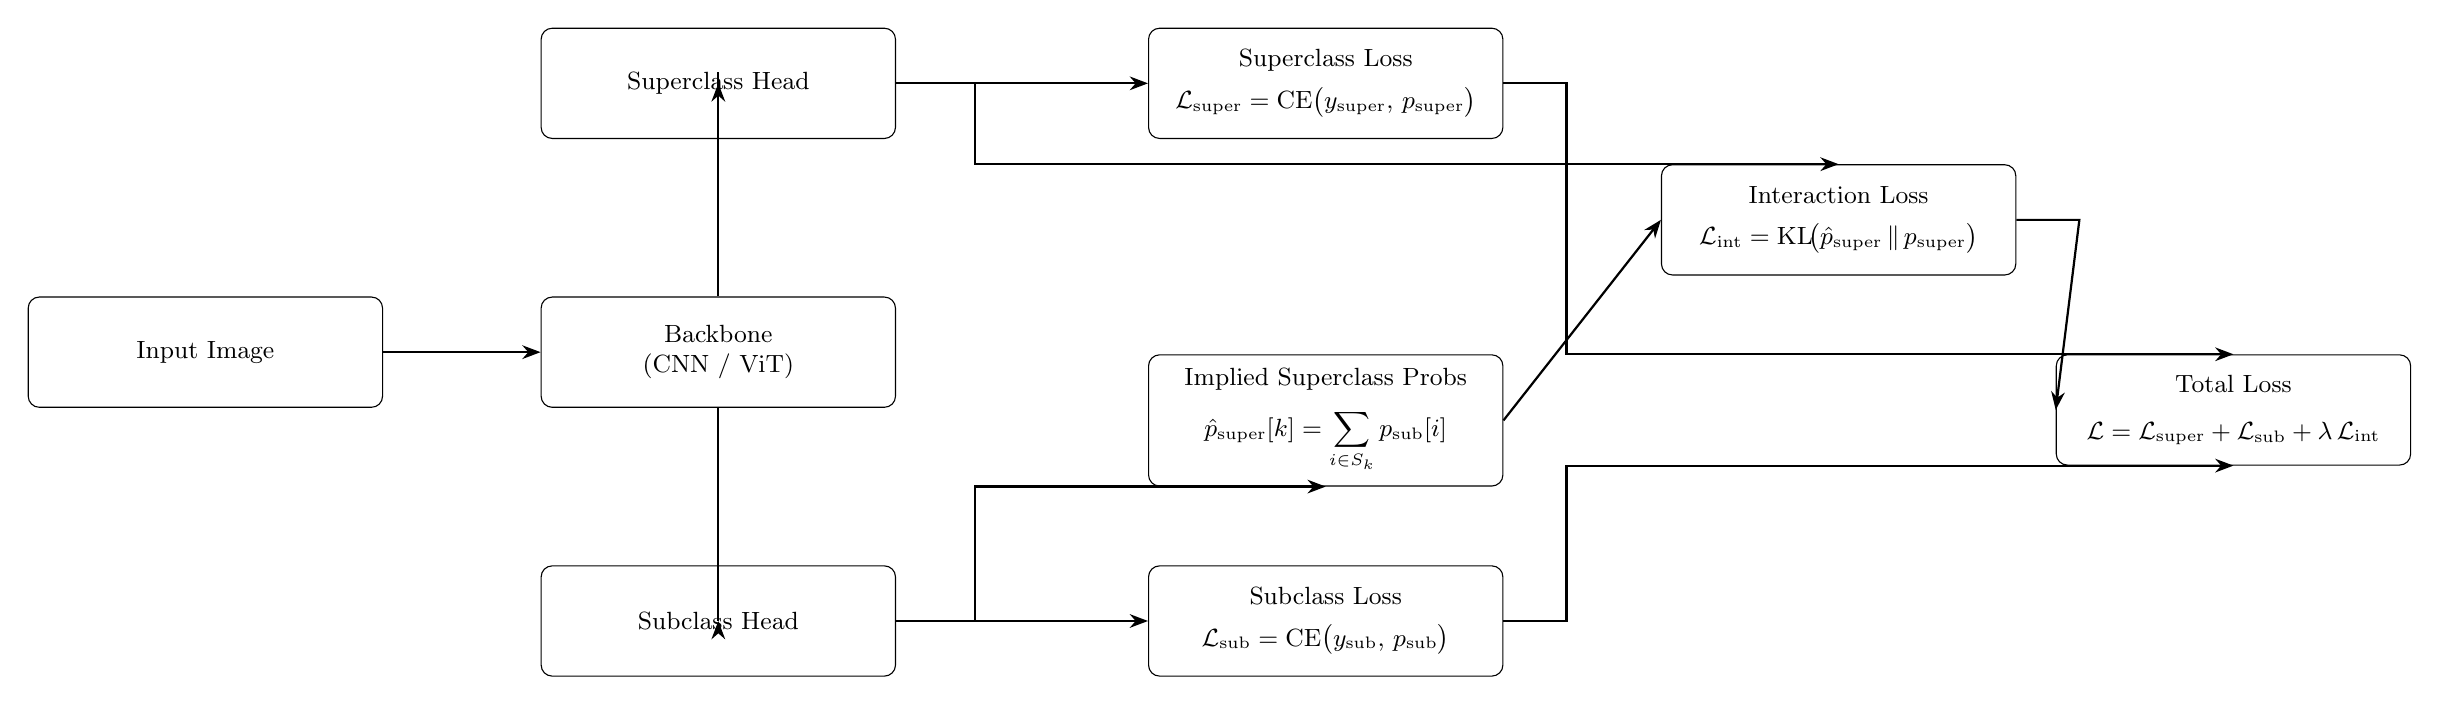
\begin{tikzpicture}[
    node distance = 2.5cm and 4.0cm,
    every node/.style={font=\small},
    box/.style={
        draw,
        rounded corners,
        align=center,
        minimum width=4.5cm,
        minimum height=1.4cm,
        inner sep=5pt
    },
    arrow/.style={-Stealth, thick}
]

% Main forward flow
\node[box] (img) {Input Image};
\node[box, right=2.0cm of img] (backbone) {Backbone\\(CNN / ViT)};

% Heads (well separated vertically)
\node[box, above=2.0cm of backbone] (superhead) {Superclass Head};
\node[box, below=2.0cm of backbone] (subhead) {Subclass Head};

% CE losses
\node[box, right=3.2cm of superhead] (Lsuper) {Superclass Loss\\[4pt]
$\mathcal{L}_{\text{super}}
 = \mathrm{CE}\big(y_{\text{super}},\, p_{\text{super}}\big)$};

\node[box, right=3.2cm of subhead] (Lsub) {Subclass Loss\\[4pt]
$\mathcal{L}_{\text{sub}}
 = \mathrm{CE}\big(y_{\text{sub}},\, p_{\text{sub}}\big)$};

% Implied superclass probabilities from subclass head
\node[box, above=1.0cm of Lsub] (qsuper) {Implied Superclass Probs\\[6pt]
$\hat p_{\text{super}}[k]
 = \displaystyle \sum_{i \in S_k} p_{\text{sub}}[i]$};

% Interaction (KL) loss: only uses implied and actual superclass probs
\node[box, above right=1.0cm and 2cm of qsuper] (Lint) {Interaction Loss\\[4pt]
$\mathcal{L}_{\text{int}}
 = \mathrm{KL}\!\big(\hat p_{\text{super}} \,\|\, p_{\text{super}}\big)$};

% Total loss (sum of the three)
\node[box, below right=1.0cm and 0.5cm of Lint] (Ltotal) {Total Loss\\[6pt]
$\mathcal{L}
 = \mathcal{L}_{\text{super}}
 + \mathcal{L}_{\text{sub}}
 + \lambda\,\mathcal{L}_{\text{int}}$};

% Main arrows
\draw[arrow] (img) -- (backbone);

\draw[arrow] (backbone) |- (superhead);
\draw[arrow] (backbone) |- (subhead);

\draw[arrow] (superhead) -- (Lsuper);
\draw[arrow] (subhead) -- (Lsub);

% From subclass head to implied superclass probs (only subclass → qsuper)
\draw[arrow] (subhead.east) -- ++(1.0,0) |- (qsuper.south);

% Interaction loss: only qsuper and superhead feed into it
\draw[arrow] (qsuper.east) -- (Lint.west);
\draw[arrow] (superhead.east) -- ++(1.0,0) |- (Lint.north);

% Contributions to total loss: all three into Ltotal
\draw[arrow] (Lsuper.east) -- ++(0.8,0) |- (Ltotal.north);
\draw[arrow] (Lsub.east)   -- ++(0.8,0) |- (Ltotal.south);
\draw[arrow] (Lint.east)   -- ++(0.8,0) -- (Ltotal.west);

\end{tikzpicture}
}
\caption{Model architecture and loss computation.}
\end{figure}

\section{Interaction Loss / KL Divergence Calculations}

For each superclass $k$, with subclass set $S_k$:
\[
\hat{p}_{\text{super}}[k]
  = \sum_{i \in S_k} p_{\text{sub}}[i].
\]

Then define interaction loss, e.g.:
\[
\mathcal{L}_{\text{int}}
  = \mathrm{KL}\!\big(\hat{p}_{\text{super}} \,\|\, p_{\text{super}}\big).
\]

The Kullback--Leibler (KL) divergence between two distributions $P$ and $Q$ is:
\[
\mathrm{KL}(P \,\|\, Q)
  = \sum_{k} P(k)\,\log \frac{P(k)}{Q(k)}.
\]


\begin{thebibliography}{99}

\bibitem{Donahue2014}
\textbf{J.~Donahue}, \textbf{Y.~Jia}, \textbf{O.~Vinyals}, \textbf{J.~Hoffman}, \textbf{N.~Zhang}, \textbf{E.~Tzeng}, and \textbf{T.~Darrell}.
DeCAF: A Deep Convolutional Activation Feature for Generic Visual Recognition.
In \emph{Proceedings of the 31st ICML}, 2014.

\bibitem{Krizhevsky2012}
\textbf{A.~Krizhevsky}, \textbf{I.~Sutskever}, and \textbf{G.~E.~Hinton}.
ImageNet Classification with Deep Convolutional Neural Networks.
In \emph{Advances in Neural Information Processing Systems (NeurIPS)}, 2012.

\bibitem{Srivastava2014}
\textbf{N.~Srivastava}, \textbf{G.~Hinton}, \textbf{A.~Krizhevsky}, \textbf{I.~Sutskever}, and \textbf{R.~Salakhutdinov}.
Dropout: A Simple Way to Prevent Neural Networks from Overfitting.
\emph{Journal of Machine Learning Research}, 15(56):1929--1958, 2014.

\bibitem{Breiman1996}
\textbf{L.~Breiman}.
Bagging predictors.
\emph{Machine Learning}, 24(2):123--140, 1996.

\bibitem{FreundSchapire1997}
\textbf{Y.~Freund} and \textbf{R.~E.~Schapire}.
A decision-theoretic generalization of on-line learning and an application to boosting.
\emph{Journal of Computer and System Sciences}, 55(1):119--139, 1997.

\bibitem{Caruana1997}
\textbf{R.~Caruana}.
Multitask Learning.
\emph{Machine Learning}, 28(1):41--75, 1997.

\bibitem{Hinton2015}
\textbf{G.~Hinton}, \textbf{O.~Vinyals}, and \textbf{J.~Dean}.
Distilling the Knowledge in a Neural Network.
In \emph{NIPS Deep Learning and Representation Learning Workshop}, 2015.

\end{thebibliography}

\end{document}
